\PassOptionsToPackage{unicode=true}{hyperref} % options for packages loaded elsewhere
\PassOptionsToPackage{hyphens}{url}
\documentclass[14pt,ignorenonframetext,]{beamer}
\setbeamertemplate{caption}[numbered]
\setbeamertemplate{caption label separator}{: }
\setbeamercolor{caption name}{fg=normal text.fg}
\beamertemplatenavigationsymbolsempty
\usepackage{lmodern}
\usepackage{amssymb,amsmath}
\usepackage{ifxetex,ifluatex}
\usepackage{fixltx2e} % provides \textsubscript
\ifnum 0\ifxetex 1\fi\ifluatex 1\fi=0 % if pdftex
  \usepackage[T1]{fontenc}
  \usepackage[utf8]{inputenc}
\else % if luatex or xelatex
  \ifxetex
    \usepackage{mathspec}
  \else
    \usepackage{fontspec}
\fi
\defaultfontfeatures{Ligatures=TeX,Scale=MatchLowercase}







\fi

  \usetheme[]{monash}

  \usecolortheme{monashblue}


% A default size of 24 is set in beamerthememonash.sty




% use upquote if available, for straight quotes in verbatim environments
\IfFileExists{upquote.sty}{\usepackage{upquote}}{}
% use microtype if available
\IfFileExists{microtype.sty}{%
  \usepackage{microtype}
  \UseMicrotypeSet[protrusion]{basicmath} % disable protrusion for tt fonts
}{}


\newif\ifbibliography


\hypersetup{
      pdftitle={Feature-based time series analysis},
        pdfauthor={Rob J Hyndman},
          pdfborder={0 0 0},
    breaklinks=true}
%\urlstyle{same}  % Use monospace font for urls




  \usepackage{color}
  \usepackage{fancyvrb}
  \newcommand{\VerbBar}{|}
  \newcommand{\VERB}{\Verb[commandchars=\\\{\}]}
  \DefineVerbatimEnvironment{Highlighting}{Verbatim}{commandchars=\\\{\}}
  % Add ',fontsize=\small' for more characters per line
  \usepackage{framed}
  \definecolor{shadecolor}{RGB}{248,248,248}
  \newenvironment{Shaded}{\begin{snugshade}}{\end{snugshade}}
  \newcommand{\AlertTok}[1]{\textcolor[rgb]{0.94,0.16,0.16}{#1}}
  \newcommand{\AnnotationTok}[1]{\textcolor[rgb]{0.56,0.35,0.01}{\textbf{\textit{#1}}}}
  \newcommand{\AttributeTok}[1]{\textcolor[rgb]{0.77,0.63,0.00}{#1}}
  \newcommand{\BaseNTok}[1]{\textcolor[rgb]{0.00,0.00,0.81}{#1}}
  \newcommand{\BuiltInTok}[1]{#1}
  \newcommand{\CharTok}[1]{\textcolor[rgb]{0.31,0.60,0.02}{#1}}
  \newcommand{\CommentTok}[1]{\textcolor[rgb]{0.56,0.35,0.01}{\textit{#1}}}
  \newcommand{\CommentVarTok}[1]{\textcolor[rgb]{0.56,0.35,0.01}{\textbf{\textit{#1}}}}
  \newcommand{\ConstantTok}[1]{\textcolor[rgb]{0.00,0.00,0.00}{#1}}
  \newcommand{\ControlFlowTok}[1]{\textcolor[rgb]{0.13,0.29,0.53}{\textbf{#1}}}
  \newcommand{\DataTypeTok}[1]{\textcolor[rgb]{0.13,0.29,0.53}{#1}}
  \newcommand{\DecValTok}[1]{\textcolor[rgb]{0.00,0.00,0.81}{#1}}
  \newcommand{\DocumentationTok}[1]{\textcolor[rgb]{0.56,0.35,0.01}{\textbf{\textit{#1}}}}
  \newcommand{\ErrorTok}[1]{\textcolor[rgb]{0.64,0.00,0.00}{\textbf{#1}}}
  \newcommand{\ExtensionTok}[1]{#1}
  \newcommand{\FloatTok}[1]{\textcolor[rgb]{0.00,0.00,0.81}{#1}}
  \newcommand{\FunctionTok}[1]{\textcolor[rgb]{0.00,0.00,0.00}{#1}}
  \newcommand{\ImportTok}[1]{#1}
  \newcommand{\InformationTok}[1]{\textcolor[rgb]{0.56,0.35,0.01}{\textbf{\textit{#1}}}}
  \newcommand{\KeywordTok}[1]{\textcolor[rgb]{0.13,0.29,0.53}{\textbf{#1}}}
  \newcommand{\NormalTok}[1]{#1}
  \newcommand{\OperatorTok}[1]{\textcolor[rgb]{0.81,0.36,0.00}{\textbf{#1}}}
  \newcommand{\OtherTok}[1]{\textcolor[rgb]{0.56,0.35,0.01}{#1}}
  \newcommand{\PreprocessorTok}[1]{\textcolor[rgb]{0.56,0.35,0.01}{\textit{#1}}}
  \newcommand{\RegionMarkerTok}[1]{#1}
  \newcommand{\SpecialCharTok}[1]{\textcolor[rgb]{0.00,0.00,0.00}{#1}}
  \newcommand{\SpecialStringTok}[1]{\textcolor[rgb]{0.31,0.60,0.02}{#1}}
  \newcommand{\StringTok}[1]{\textcolor[rgb]{0.31,0.60,0.02}{#1}}
  \newcommand{\VariableTok}[1]{\textcolor[rgb]{0.00,0.00,0.00}{#1}}
  \newcommand{\VerbatimStringTok}[1]{\textcolor[rgb]{0.31,0.60,0.02}{#1}}
  \newcommand{\WarningTok}[1]{\textcolor[rgb]{0.56,0.35,0.01}{\textbf{\textit{#1}}}}


  \usepackage{graphicx,grffile}
  \makeatletter
  \def\maxwidth{\ifdim\Gin@nat@width>\linewidth\linewidth\else\Gin@nat@width\fi}
  \def\maxheight{\ifdim\Gin@nat@height>\textheight0.8\textheight\else\Gin@nat@height\fi}
  \makeatother
  % Scale images if necessary, so that they will not overflow the page
  % margins by default, and it is still possible to overwrite the defaults
  % using explicit options in \includegraphics[width, height, ...]{}
  \setkeys{Gin}{width=\maxwidth,height=\maxheight,keepaspectratio}

% Prevent slide breaks in the middle of a paragraph:
\widowpenalties 1 10000
\raggedbottom

  \AtBeginPart{
    \let\insertpartnumber\relax
    \let\partname\relax
    \frame{\partpage}
  }
  \AtBeginSection{
    \ifbibliography
    \else
      \let\insertsectionnumber\relax
      \let\sectionname\relax
      \frame{\sectionpage}
    \fi
  }
  \AtBeginSubsection{
    \let\insertsubsectionnumber\relax
    \let\subsectionname\relax
    \frame{\subsectionpage}
  }



\setlength{\parindent}{0pt}
\setlength{\parskip}{6pt plus 2pt minus 1pt}
\setlength{\emergencystretch}{3em}  % prevent overfull lines
\providecommand{\tightlist}{%
  \setlength{\itemsep}{0pt}\setlength{\parskip}{0pt}}

  \setcounter{secnumdepth}{0}


  \usepackage{ragged2e,booktabs,multicol}
  \graphicspath{{figs/}}
  \usepackage{bm}
  \def\Var{\text{Var}}
  \newcommand{\X}{\mathbf{X}}
  \newcommand{\x}{\mathbf{x}}
  \renewcommand{\H}{\mathbf{H}}
  
  \fontsize{13}{15}\sf
  \usepackage[scale=0.85]{sourcecodepro}
  \DisableLigatures{encoding = T1, family = tt*}
  
  \def\full#1{\vspace*{0.2cm}\par\centerline{\includegraphics[height=8.1cm,width=12.8cm,keepaspectratio=true]{#1}}}
  
  \definecolor{ao(english)}{rgb}{0.0, 0.5, 0.0}
  
  \definecolor{aureolin}{rgb}{0.99, 0.93, 0.0}

%% Monash overrides
\AtBeginSection[]{
   \frame<beamer>{
   \frametitle{Outline}
   \tableofcontents[currentsection,hideallsubsections]
  }}
% Redefine shaded environment if it exists (to ensure text is black)
\ifcsname Shaded\endcsname
  \definecolor{shadecolor}{RGB}{225,225,225}
  \renewenvironment{Shaded}{\color{black}\begin{snugshade}\color{black}}{\end{snugshade}}
\fi
%%

  \title[]{Feature-based time series analysis}


  \author[
        Rob J Hyndman
    ]{Rob J Hyndman}


\date[
      26 November 2018
  ]{
      26 November 2018
        }

\begin{document}

% Hide progress bar and footline on titlepage
  \begin{frame}[plain]
  \titlepage
  \end{frame}


   \frame<beamer>{
   \frametitle{Outline}
   \tableofcontents[hideallsubsections]
  }

\hypertarget{visualization}{%
\section{Visualization}\label{visualization}}

\begin{frame}{M3 competition}
\protect\hypertarget{m3-competition}{}

\full{M3paper}
\only<2>{
\placefig{1}{4}{height=3cm, width=10cm, keepaspectratio=true}{SMakridakis}
\placefig{8.8}{4}{height=3cm, width=10cm, keepaspectratio=true}{MHibon}}

\end{frame}

\begin{frame}{How to plot lots of time series?}
\protect\hypertarget{how-to-plot-lots-of-time-series}{}

\only<1>{\full{M3data1}}
\only<2>{\full{M3data2}}
\only<3>{\full{M3data3}}
\only<4>{\full{M3data4}}
\only<5>{\full{M3data5}}
\only<6>{\full{M3data10}}
\only<7>{\full{M3data20}}
\only<8>{\full{M3data30}}
\only<9>{\full{M3data40}}
\only<10>{\full{M3data50}}
\only<11>{\full{M3data100}}
\only<12>{\full{M3data200}}
\only<13>{\full{M3data500}}
\only<14>{\full{M3data3003}}

\end{frame}

\begin{frame}{Key idea}
\protect\hypertarget{key-idea}{}

\placefig{9.1}{.5}{width=3.6cm}{tukey}
\begin{textblock}{3}(9.7,5.4)\small\textit{John W Tukey}\end{textblock}
\begin{textblock}{8}(0.7,1.2)
\begin{alertblock}{Cognostics}
Computer-produced diagnostics\\ (Tukey and Tukey, 1985).
\end{alertblock}
\end{textblock}\pause
\vspace*{2.5cm}

\alert{Examples for time series}

\begin{itemize}
\tightlist
\item
  lag correlation
\item
  size and direction of trend
\item
  strength of seasonality
\item
  timing of peak seasonality
\item
  spectral entropy
\end{itemize}

\vspace*{0.3cm}
\begin{block}{}
Called ``features'' in the machine learning literature.
\end{block}

\end{frame}

\begin{frame}{An STL decomposition: N2096}
\protect\hypertarget{an-stl-decomposition-n2096}{}

\begin{alertblock}{}
\centerline{$Y_t = S_t + T_t + R_t$\qquad $S_{t}$ is periodic with mean 0}
\end{alertblock}

\includegraphics{fbtsa_monash_files/figure-beamer/stl-1.pdf}

\end{frame}

\begin{frame}{Candidate features}
\protect\hypertarget{candidate-features}{}

\begin{block}{STL decomposition}
\centerline{$Y_t = S_t + T_t + R_t$}
\end{block}\pause\fontsize{14}{16}\sf\vspace*{-0.2cm}

\begin{itemize}
\tightlist
\item
  Seasonal period
\item
  Autocorrelations of data (\(Y_1,\dots,Y_T\))
\item
  Autocorrelations of data (\(R_1,\dots,R_T\))
\item
  Strength of seasonality:
  \(\max\left(0,1 - \frac{\Var(R_t)}{\Var(Y_t-T_t)}\right)\)
\item
  Strength of trend:
  \(\max\left(0,1 - \frac{\Var(R_t)}{\Var(Y_t-S_t)}\right)\)
\item
  Spectral entropy:
  \(H = - \int_{-\pi}^{\pi} f_y(\lambda) \log f_y(\lambda) d\lambda\),
  where \(f_y(\lambda)\) is spectral density of \(Y_t\).\newline Low
  values of \(H\) suggest a time series that is easier to forecast (more
  signal).
\item
  Optimal Box-Cox transformation of data
\end{itemize}

\fontsize{9}{10}\sf

\end{frame}

\begin{frame}{Distribution of Period for M3}
\protect\hypertarget{distribution-of-period-for-m3}{}

\includegraphics{fbtsa_monash_files/figure-beamer/M3period-1.pdf}

\end{frame}

\begin{frame}{Distribution of Seasonality for M3}
\protect\hypertarget{distribution-of-seasonality-for-m3}{}

\includegraphics{fbtsa_monash_files/figure-beamer/M3season-1.pdf}

\only<2->{
\begin{textblock}{6}(0.2,3)
  \begin{alertblock}{Low Seasonality}
    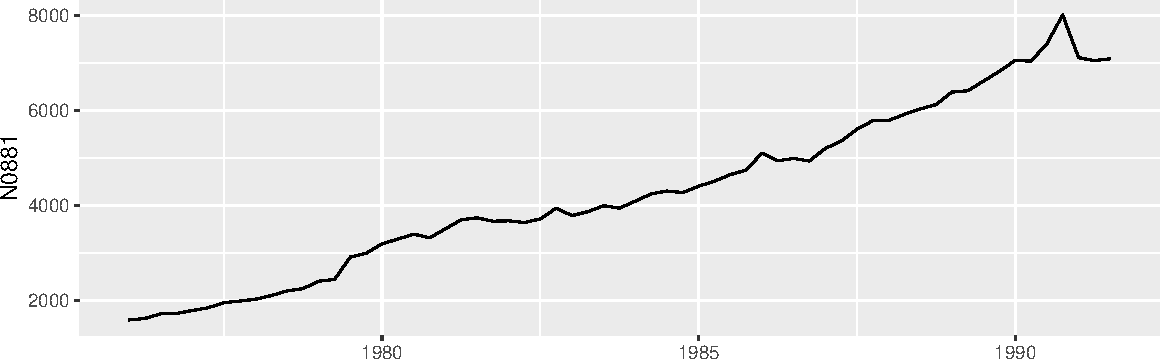
\includegraphics[width=6cm]{M3seasonLo.pdf}
  \end{alertblock}
\end{textblock}
}
\only<3>{
\begin{textblock}{6}(6.6,3)
  \begin{alertblock}{High Seasonality}
    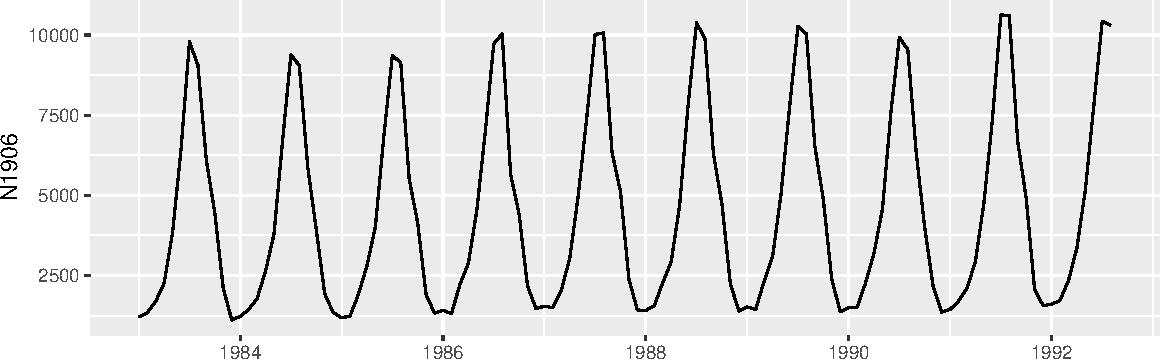
\includegraphics[width=6cm]{M3seasonHi.pdf}
  \end{alertblock}
\end{textblock}
}

\end{frame}

\begin{frame}{Distribution of Trend for M3}
\protect\hypertarget{distribution-of-trend-for-m3}{}

\includegraphics{fbtsa_monash_files/figure-beamer/M3trend-1.pdf}

\only<2->{
\begin{textblock}{6}(0.2,3)
  \begin{alertblock}{Low Trend}
    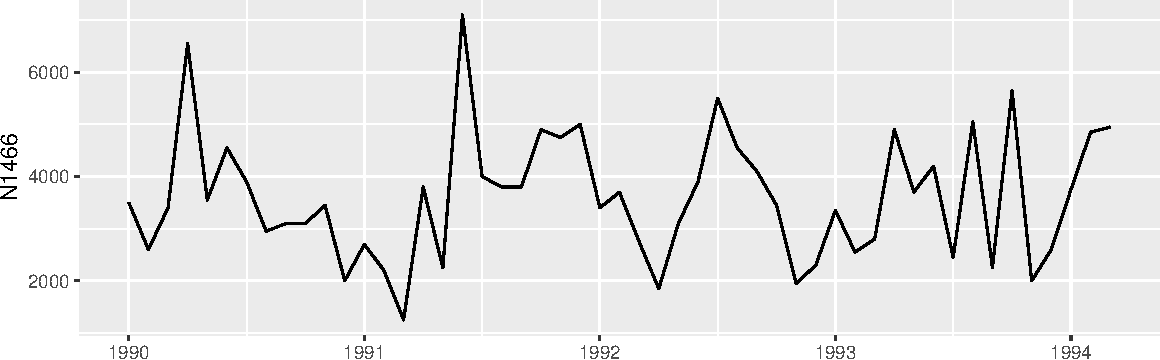
\includegraphics[width=6cm]{M3trendLo.pdf}
  \end{alertblock}
\end{textblock}
}
\only<3>{
\begin{textblock}{6}(6.6,3)
  \begin{alertblock}{High Trend}
    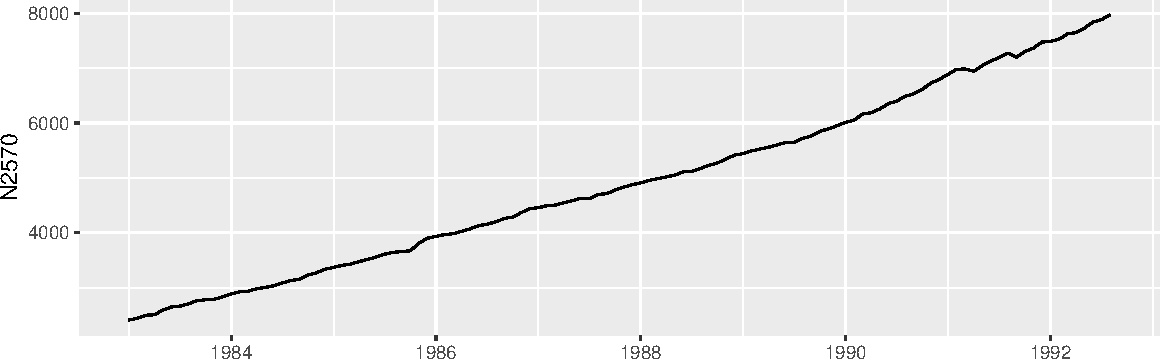
\includegraphics[width=6cm]{M3trendHi.pdf}
  \end{alertblock}
\end{textblock}
}

\end{frame}

\begin{frame}{Distribution of Residual ACF1 for M3}
\protect\hypertarget{distribution-of-residual-acf1-for-m3}{}

\includegraphics{fbtsa_monash_files/figure-beamer/M3ACF1-1.pdf}

\only<2->{
\begin{textblock}{6}(0.2,3)
  \begin{alertblock}{Low ACF1}
    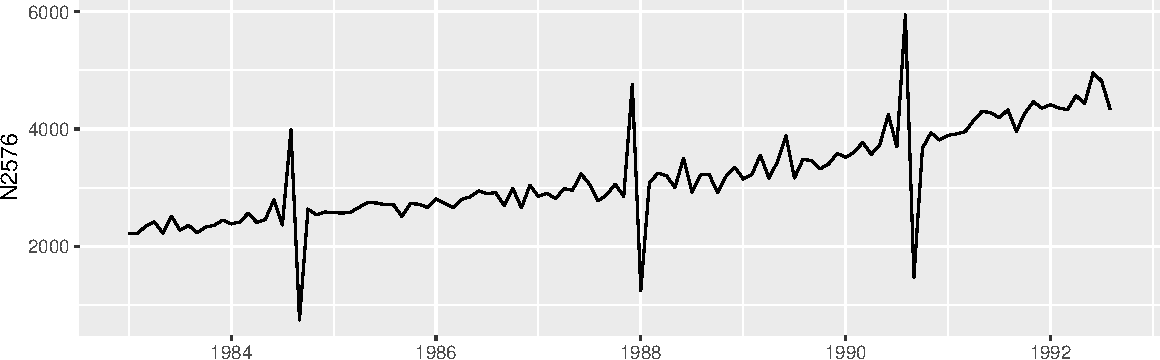
\includegraphics[width=6cm]{M3acfLo.pdf}
  \end{alertblock}
\end{textblock}
}
\only<3>{
\begin{textblock}{6}(6.6,3)
  \begin{alertblock}{High ACF1}
    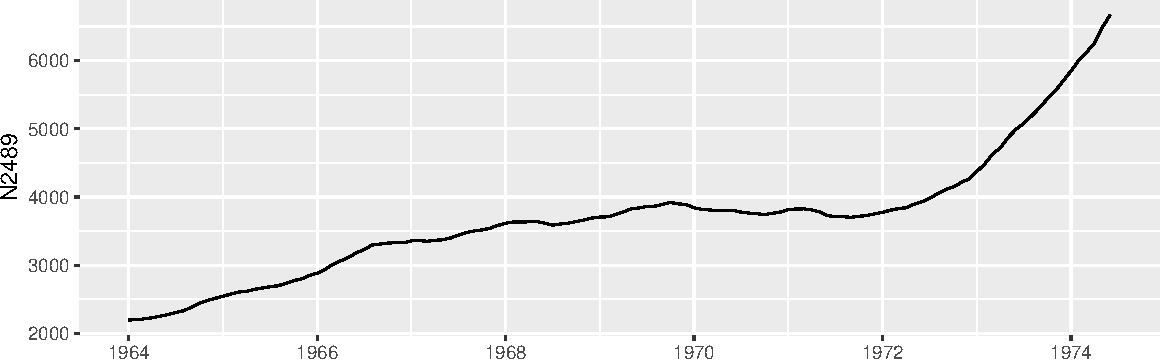
\includegraphics[width=6cm]{M3acfHi.pdf}
  \end{alertblock}
\end{textblock}
}

\end{frame}

\begin{frame}{Distribution of Spectral Entropy for M3}
\protect\hypertarget{distribution-of-spectral-entropy-for-m3}{}

\includegraphics{fbtsa_monash_files/figure-beamer/M3entropy-1.pdf}

\only<2->{
\begin{textblock}{6}(0.2,3)
  \begin{alertblock}{Low Entropy}
    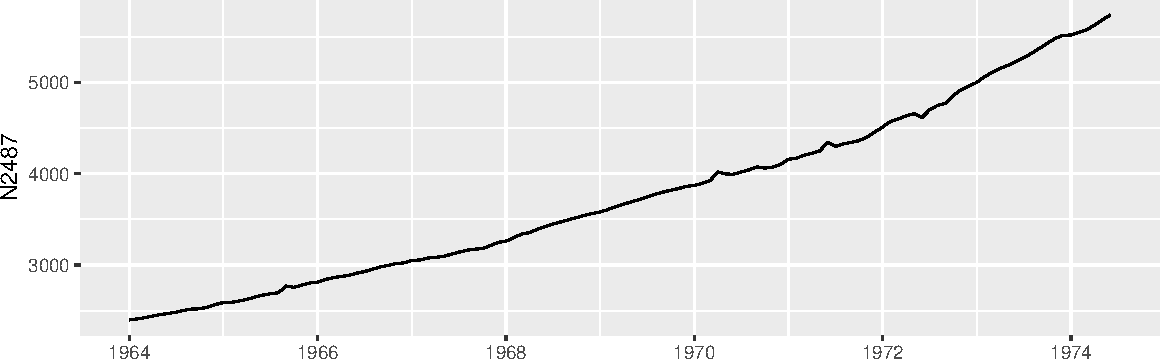
\includegraphics[width=6cm]{M3specLo.pdf}
  \end{alertblock}
\end{textblock}
}
\only<3>{
\begin{textblock}{6}(6.6,3)
  \begin{alertblock}{High Entropy}
    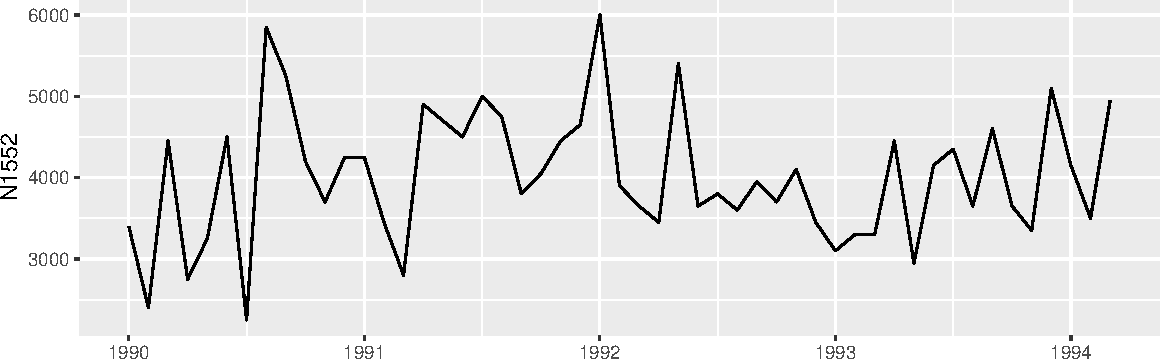
\includegraphics[width=6cm]{M3specHi.pdf}
  \end{alertblock}
\end{textblock}
}

\end{frame}

\begin{frame}{Feature distributions}
\protect\hypertarget{feature-distributions}{}

\includegraphics{fbtsa_monash_files/figure-beamer/ACF1SE-1.pdf}

\end{frame}

\begin{frame}{Feature distributions}
\protect\hypertarget{feature-distributions-1}{}

\includegraphics{fbtsa_monash_files/figure-beamer/TrendSE-1.pdf}

\end{frame}

\begin{frame}{Feature distributions}
\protect\hypertarget{feature-distributions-2}{}

\includegraphics{fbtsa_monash_files/figure-beamer/M3pairs-1.pdf}

\end{frame}

\begin{frame}{Dimension reduction for time series}
\protect\hypertarget{dimension-reduction-for-time-series}{}

\only<1->{\placefig{0}{1}{width=4cm,height=8.3cm,trim=0 0 200 0,clip=TRUE}{M3sample}}
\only<2->{\placefig{6}{1}{width=6cm}{PairwisePlot}}
\only<3>{\placefig{5.2}{5.3}{width=5cm}{FeatureSpace}}

\only<2->{\placefig{4}{2}{width=2cm}{arrow}}
\only<3>{\placefig{8.4}{4.2}{width=2cm,angle=-90}{arrow}}

\only<2->{\begin{textblock}{2.1}(4,2.6)
\begin{alertblock}{}\small
Feature calculation
\end{alertblock}
\end{textblock}}

\only<3->{\begin{textblock}{2.8}(9.7,4.1)
\begin{alertblock}{}\small
Principal component decomposition
\end{alertblock}
\end{textblock}}

\end{frame}

\begin{frame}{M3 feature space}
\protect\hypertarget{m3-feature-space}{}

\fontsize{11}{11}\sf

\vspace*{-0.2cm}

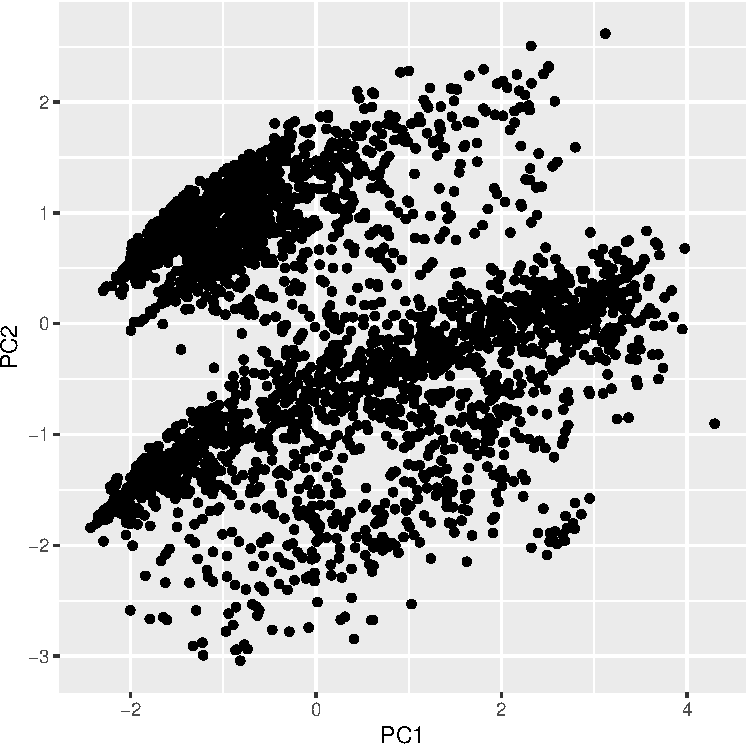
\includegraphics[width=8.2cm]{FeatureSpace}

\begin{textblock}{4}(8,3)
\begin{block}{}\fontsize{12}{13}\sf
First two PCs explain 58.5\% of the variance.
\end{block}
\end{textblock}

\end{frame}

\begin{frame}{M3 feature space}
\protect\hypertarget{m3-feature-space-1}{}

\includegraphics{fbtsa_monash_files/figure-beamer/m3biplot-1.pdf}

\end{frame}

\begin{frame}{M3 feature space}
\protect\hypertarget{m3-feature-space-2}{}

\includegraphics{fbtsa_monash_files/figure-beamer/m3pca1-1.pdf}

\end{frame}

\begin{frame}{Feature properties}
\protect\hypertarget{feature-properties}{}

In this analysis, we have restricted features to be

\begin{itemize}
\tightlist
\item
  ergodic
\item
  scale-independent
\end{itemize}

For other analyses, it may be appropriate to have different
requirements.

\end{frame}

\begin{frame}[fragile]{R package: tsfeatures}
\protect\hypertarget{r-package-tsfeatures}{}

\alert{github.com/robjhyndman/tsfeatures}\fontsize{9.5}{11}\sf

\begin{Shaded}
\begin{Highlighting}[]
\KeywordTok{library}\NormalTok{(tsfeatures)}
\KeywordTok{library}\NormalTok{(tidyverse)}
\KeywordTok{library}\NormalTok{(forecast)}

\NormalTok{myfeatures <-}\StringTok{ }\ControlFlowTok{function}\NormalTok{(x,...) \{}
\NormalTok{  lambda <-}\StringTok{ }\KeywordTok{BoxCox.lambda}\NormalTok{(x, }\DataTypeTok{lower=}\DecValTok{0}\NormalTok{, }\DataTypeTok{upper=}\DecValTok{1}\NormalTok{, }\DataTypeTok{method=}\StringTok{'loglik'}\NormalTok{)}
\NormalTok{  y <-}\StringTok{ }\KeywordTok{BoxCox}\NormalTok{(x, lambda)}
  \KeywordTok{c}\NormalTok{(}\KeywordTok{stl_features}\NormalTok{(y,}\DataTypeTok{s.window=}\StringTok{'periodic'}\NormalTok{, }\DataTypeTok{robust=}\OtherTok{TRUE}\NormalTok{, ...),}
    \DataTypeTok{lambda=}\NormalTok{lambda)}
\NormalTok{\}}
\NormalTok{M3Features <-}\StringTok{ }\KeywordTok{bind_cols}\NormalTok{(}
  \KeywordTok{tsfeatures}\NormalTok{(M3data, }\KeywordTok{c}\NormalTok{(}\StringTok{"frequency"}\NormalTok{, }\StringTok{"entropy"}\NormalTok{)),}
  \KeywordTok{tsfeatures}\NormalTok{(M3data, }\StringTok{"myfeatures"}\NormalTok{, }\DataTypeTok{scale=}\OtherTok{FALSE}\NormalTok{))}
\end{Highlighting}
\end{Shaded}

\end{frame}

\hypertarget{forecasting}{%
\section{Forecasting}\label{forecasting}}

\begin{frame}{Forecast model selection}
\protect\hypertarget{forecast-model-selection}{}

\alert{Features used to select a forecasting model}\vspace*{10cm}

\begin{textblock}{12}(0.1,2.1)\small
\begin{multicols}{2}
  \begin{itemize}\tightlist
    \item length
    \item strength of seasonality
    \item strength of trend
    \item linearity
    \item curvature
    \item spikiness
    \item stability
    \item lumpiness
    \item first ACF value of remainder series
    \item parameter estimates of Holt's linear trend method
    \item spectral entropy
    \item Hurst exponent
    \item nonlinearity
    \item parameter estimates of Holt-Winters' additive method
    \item unit root test statistics
    \item first ACF value of residual series of linear trend model
    \item ACF and PACF based features - calculated on both the raw and differenced series
    \end{itemize}
\end{multicols}
\end{textblock}

\end{frame}

\begin{frame}{\fontsize{16}{16}\bf\sffamily FFORMS: Feature-based FORecast Model Selection}
\protect\hypertarget{section}{}

\only<1>{\full{fw1}}
\only<2>{\full{fw2}}
\only<3>{\full{fw3}}
\only<4>{\full{fw4}}
\only<5>{\full{fw5}}
\only<6>{\full{fw6}}
\only<7>{\full{fw7}}
\only<8>{\full{fw8}}
\only<9>{\full{fw9}}
\only<10>{\full{fw10}}
\only<11>{\full{fw11}}
\only<12>{\full{fw12}}
\only<13>{\full{fw13}}
\only<14>{\full{fw14}}

\vspace*{10cm}

\end{frame}

\begin{frame}{Application to M competition data}
\protect\hypertarget{application-to-m-competition-data}{}

\begin{block}{Experiment 1}
\centering\small\tabcolsep=0.1cm
\begin{tabular}{lrrrrr}
                 & Source & Y      & Q      & M \\
\midrule
Observed series  & M1     & 181    & 203    & 617 \\
Simulated series &        & 362000 & 406000 & 123400 \\
New series       & M3     & 645    & 756    & 1428
\end{tabular}
\end{block}
\begin{block}{Experiment 2}
\centering\small\tabcolsep=0.1cm
\begin{tabular}{lrrrrr}
                 & Source & Y       & Q       & M \\
\midrule
Observed series  & M3     & 645     & 756     & 1428 \\
Simulated series &        & 1290000 & 1512000 & 285600 \\
New series       & M1     & 181     & 203     & 617
\end{tabular}
\end{block}

\end{frame}

\begin{frame}{Results: Yearly}
\protect\hypertarget{results-yearly}{}

\includegraphics{fbtsa_monash_files/figure-beamer/unnamed-chunk-1-1.pdf}

\end{frame}

\begin{frame}{Results: Quarterly}
\protect\hypertarget{results-quarterly}{}

\includegraphics{fbtsa_monash_files/figure-beamer/unnamed-chunk-2-1.pdf}

\end{frame}

\begin{frame}{Results: Monthly}
\protect\hypertarget{results-monthly}{}

\includegraphics{fbtsa_monash_files/figure-beamer/unnamed-chunk-3-1.pdf}

\end{frame}

\begin{frame}{\fontsize{15}{15}\sffamily\bfseries FFORMA: Feature-based FORecast Model Averaging}
\protect\hypertarget{section-1}{}

\begin{itemize}
\tightlist
\item
  Like FFORMS but we use xgboost rather than a random forest.
\item
  The optimization criterion is forecast accuracy not classification
  accuracy.
\item
  The probability of each model being best is used to construct a model
  weight.
\item
  A combination forecast is produced using these weights.
\item
  \alert{Came second in the M4 competition}
\end{itemize}

\end{frame}

\begin{frame}{\fontsize{15}{15}\sffamily\bfseries FFORMA: Feature-based FORecast Model Averaging}
\protect\hypertarget{section-2}{}

\begin{block}{Models included}

\begin{enumerate}
\tightlist
\item
  Naive
\item
  Seasonal naive
\item
  Random walk with drift
\item
  Theta method
\item
  ARIMA
\item
  ETS
\item
  TBATS
\item
  STLM-AR
\end{enumerate}

\end{block}

\end{frame}

\begin{frame}{R Packages}
\protect\hypertarget{r-packages}{}

\fontsize{14.5}{19}\sf

\begin{itemize}
\item
  \alert{seer}: FFORMS --- selecting forecasting model using features.
  \newline\url{github.com/thiyangt/seer}\vspace*{0.5cm}
\item
  \alert{M4metalearning}: FFORMA -- forecast combinations using features
  to choose weights. \newline\url{github.com/robjhyndman/M4metalearning}
\end{itemize}

\end{frame}

\hypertarget{anomaly-detection}{%
\section{Anomaly detection}\label{anomaly-detection}}

\begin{frame}{Yahoo server metrics}
\protect\hypertarget{yahoo-server-metrics}{}

\fontsize{13}{15}\sf\vspace*{-0.2cm}

\begin{itemize}
\tightlist
\item
  Tens of thousands of time series collected at one-hour intervals over
  1--2 months.
\item
  Consisting of several server metrics (e.g.~CPU usage and paging views)
  from many server farms globally.
\item
  Aim: find unusual (anomalous) time series.
\end{itemize}

\placefig{0}{4.6}{width=13.7cm, trim=0 20 0 220, clip=TRUE}{serverfarm}
\vspace*{10cm}

\end{frame}

\begin{frame}{Yahoo server metrics}
\protect\hypertarget{yahoo-server-metrics-1}{}

\vspace*{0.2cm}\par

\only<1>{\centerline{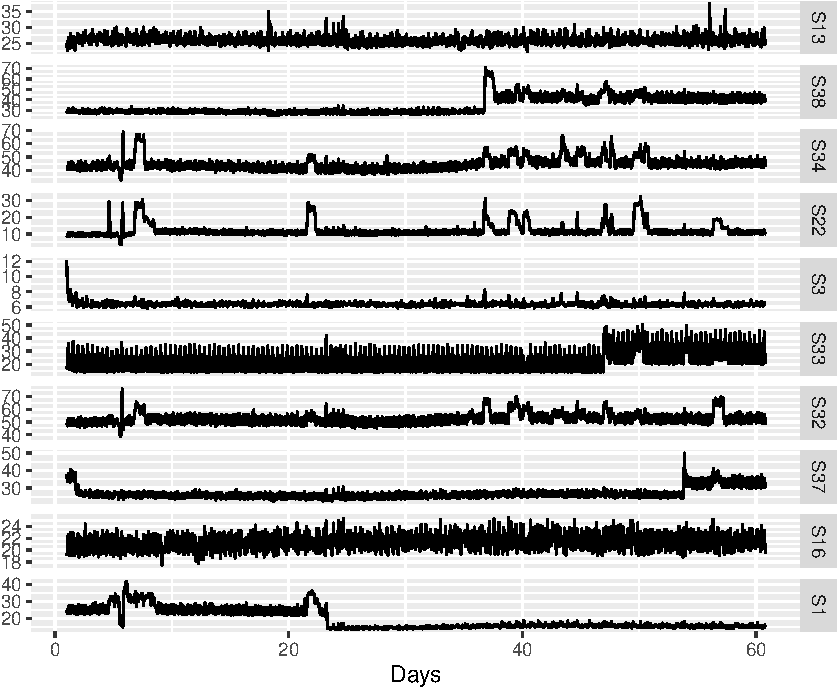
\includegraphics[height=8.1cm,width=12.8cm,keepaspectratio=true,
clip=true,trim=40 0 0 0]{yahoodata1}}}
\only<2>{\centerline{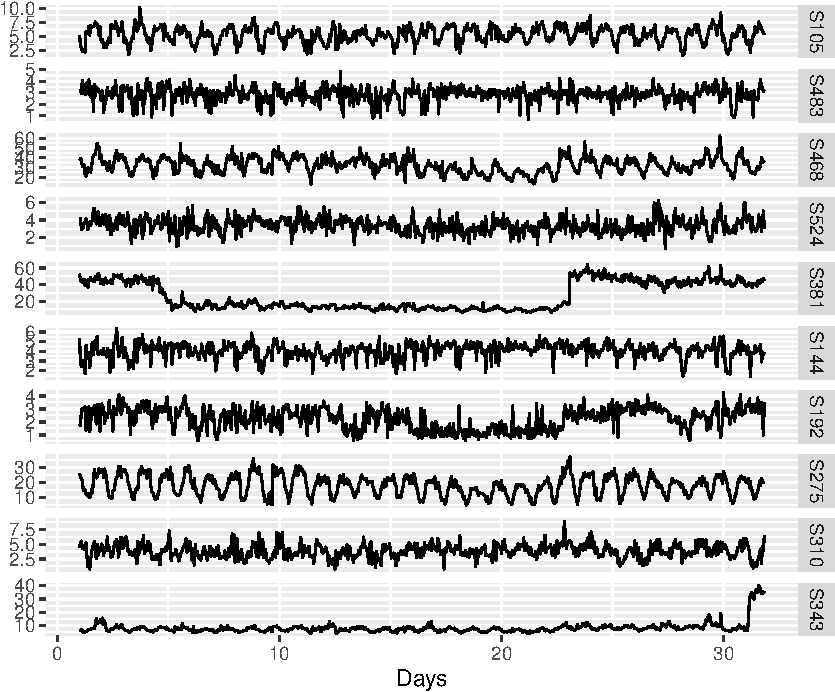
\includegraphics[height=8.1cm,width=12.8cm,keepaspectratio=true,
clip=true,trim=40 0 0 0]{yahoodata2}}}
\only<3>{\centerline{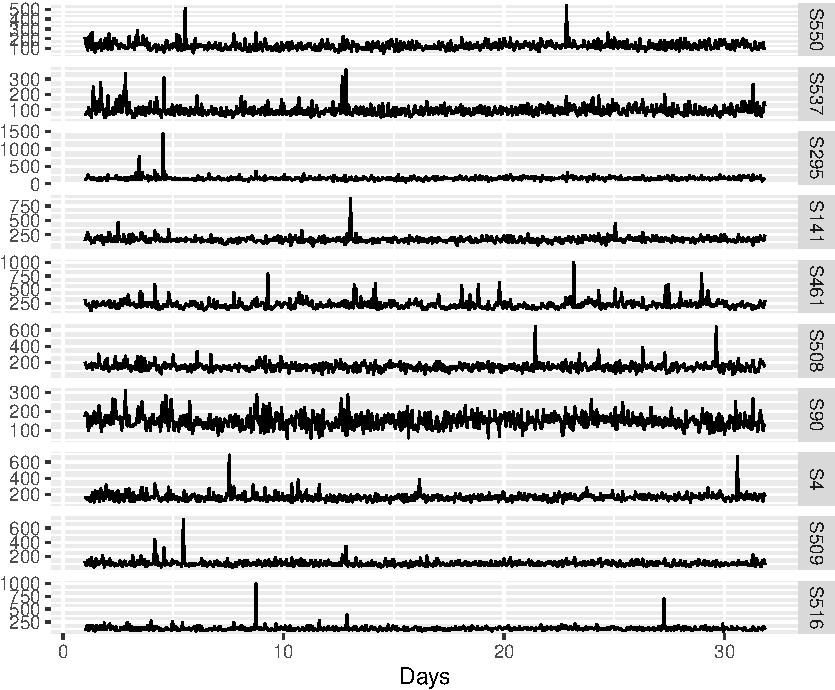
\includegraphics[height=8.1cm,width=12.8cm,keepaspectratio=true,
clip=true,trim=40 0 0 0]{yahoodata3}}}

\end{frame}

\begin{frame}{Yahoo server metrics}
\protect\hypertarget{yahoo-server-metrics-2}{}

\fontsize{11}{11.8}\sf\vspace*{-0.2cm}

\begin{itemize}
\tightlist
\item
  \textbf{ACF1}: first order autocorrelation =
  \(\text{Corr}(Y_t,Y_{t-1})\)
\item
  Strength of \textbf{trend} and \textbf{seasonality} based on STL
\item
  Size of seasonal \textbf{peak} and \textbf{trough}
\item
  Spectral \textbf{entropy}
\item
  \textbf{Lumpiness}: variance of block variances (block size 24).
\item
  \textbf{Spikiness}: variances of leave-one-out variances of STL
  remainders.
\item
  \textbf{Level shift}: Maximum difference in trimmed means of
  consecutive moving windows of size 24.
\item
  \textbf{Variance change}: Max difference in variances of consecutive
  moving windows of size 24.
\item
  \textbf{Flat spots}: Discretize sample space into 10 equal-sized
  intervals. Find max run length in any interval.
\item
  Number of \textbf{crossing points} of mean line.
\item
  \textbf{Kullback-Leibler score}: Maximum of
  \(D_{KL}(P\|Q) = \int P(x)\ln P(x)/ Q(x) dx\) where \(P\) and \(Q\)
  are estimated by kernel density estimators applied to consecutive
  windows of size 48.
\item
  \textbf{Change index}: Time of maximum KL score
\end{itemize}

\end{frame}

\begin{frame}{Feature space}
\protect\hypertarget{feature-space}{}

\fontsize{11}{11}\sf

\vspace*{-0.2cm}

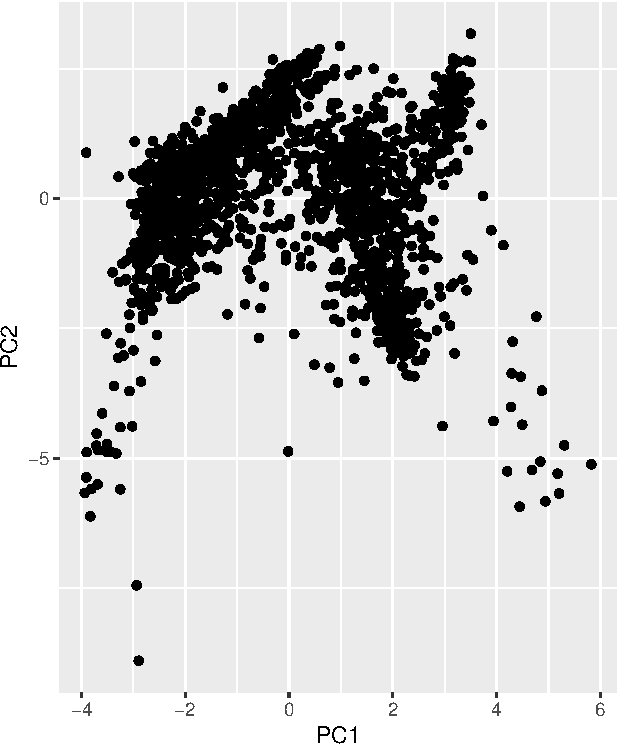
\includegraphics[width=5.8cm]{YahooFeatureSpace}

\end{frame}

\begin{frame}{Feature space}
\protect\hypertarget{feature-space-1}{}

\includegraphics{fbtsa_monash_files/figure-beamer/yahoobiplot-1.pdf}

\only<2>{\begin{textblock}{4}(8,3)\fontsize{11}{11}\sf
\begin{alertblock}{\fontsize{11}{11}\sffamily What is ``anomalous''?}
\begin{itemize}\tightlist
\item We need a measure of the ``anomalousness'' of a time series.
\item Rank points based on their local density using a bivariate kernel density estimate.
\end{itemize}
\end{alertblock}
\end{textblock}}

\end{frame}

\begin{frame}[fragile]{Finding weird time series}
\protect\hypertarget{finding-weird-time-series}{}

\fontsize{10}{10}\sf

\begin{Shaded}
\begin{Highlighting}[]
\NormalTok{hdrcde}\OperatorTok{::}\KeywordTok{hdrscatterplot}\NormalTok{(pc[,}\DecValTok{1}\NormalTok{], pc[,}\DecValTok{2}\NormalTok{], }\DataTypeTok{noutliers=}\DecValTok{5}\NormalTok{)}
\end{Highlighting}
\end{Shaded}

\vspace*{-0.25cm}

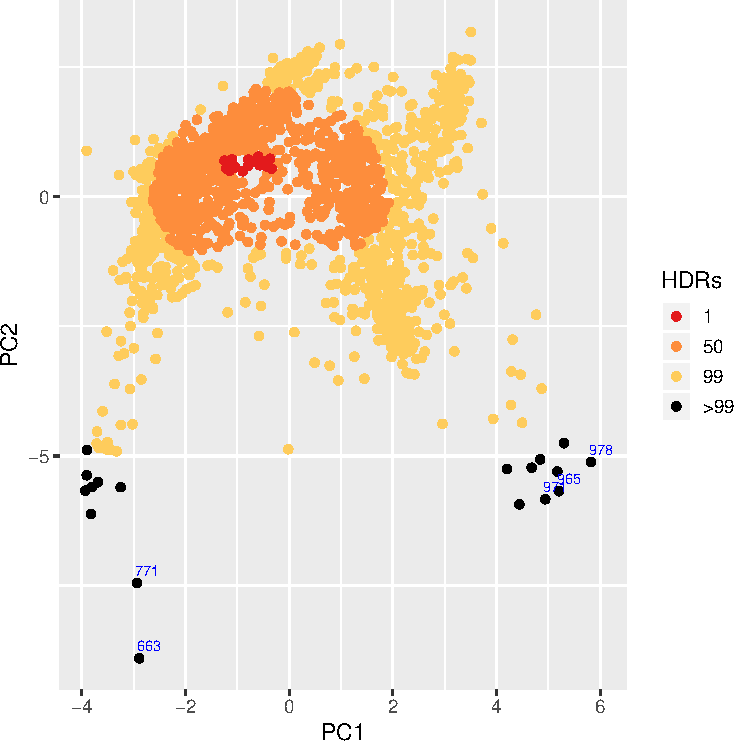
\includegraphics[width=7.5cm]{HDRYahoo}

\begin{textblock}{4.8}(7.7,6.9)\fontsize{10}{10}\sf
\begin{alertblock}{\fontsize{10}{10}\sffamily Highest Density Regions}
\begin{itemize}\tightlist
\item Estimate using \texttt{hdrcde} package
\item Highlight outlying points as those with lowest density.
\end{itemize}
\end{alertblock}
\end{textblock}

\end{frame}

\begin{frame}{Packages}
\protect\hypertarget{packages}{}

\fontsize{14.5}{18}\sf

\begin{itemize}
\item
  \alert{hdrcde}: scatterplots with bivariate HDRs. \newline CRAN
  \textbar{} \url{github.com/robjhyndman/hdrcde}\vspace*{0.4cm}
\item
  \alert{stray}: finding outliers in high dimensions.
  \newline\url{github.com/pridiltal/stray}\vspace*{0.4cm}
\item
  \alert{oddstream}: finding outliers in streaming data.
  \newline\url{github.com/pridiltal/oddstream}\vspace*{0.4cm}
\item
  \alert{anomalous}: yahoo data.
  \newline\url{github.com/robjhyndman/anomalous}
\end{itemize}

\end{frame}

\begin{frame}{Acknowledgments}
\protect\hypertarget{acknowledgments}{}

\begin{block}{}

\fontsize{11}{11}\sf

\centering

\begin{tabular}{p{3.2cm}p{3.4cm}p{3.4cm}}
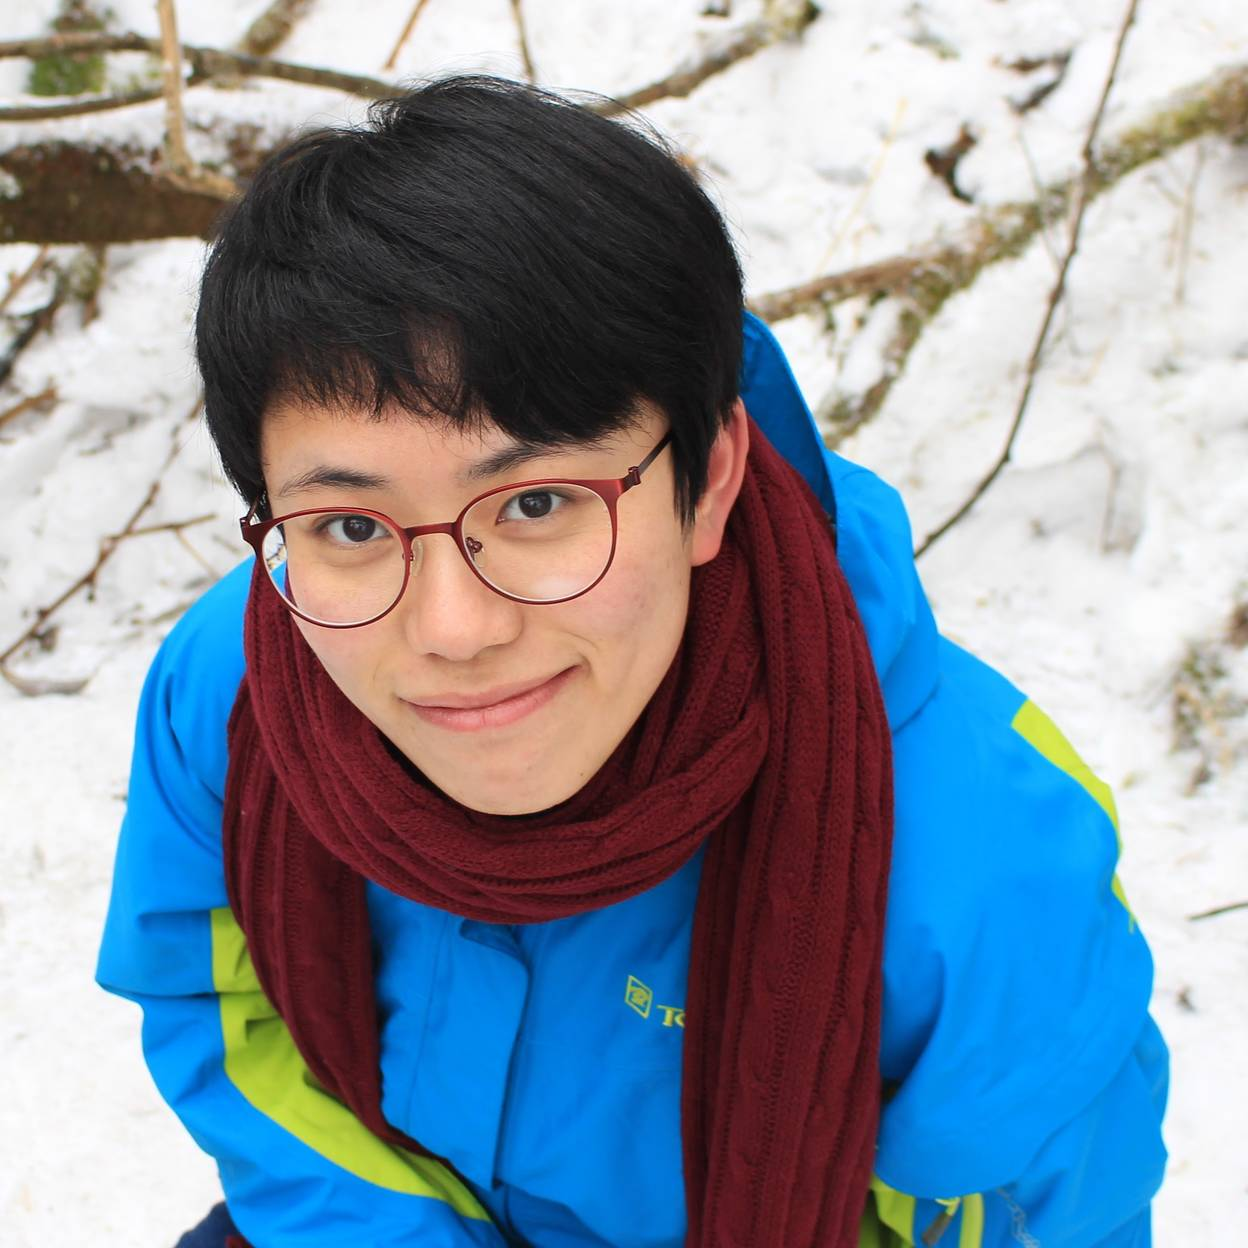
\includegraphics[height=3cm, width=10cm, keepaspectratio]{earowang} &
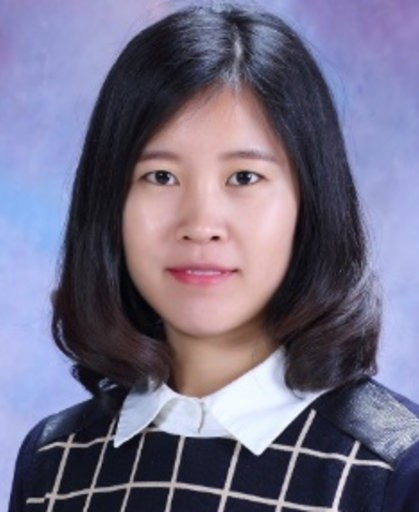
\includegraphics[height=3cm, width=10cm, keepaspectratio]{yanfei} &
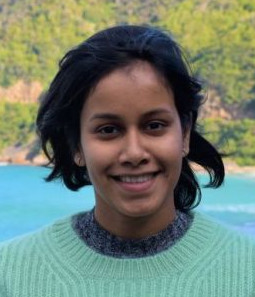
\includegraphics[height=3cm, width=10cm, keepaspectratio]{dilini}\\
Earo Wang  & Yanfei Kang & Dilini Talagala \\
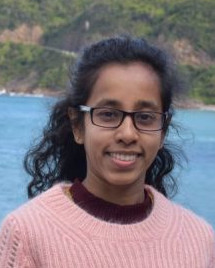
\includegraphics[height=3cm, width=10cm, keepaspectratio]{thiyanga} &

\includegraphics[height=3cm, width=10cm, keepaspectratio]{pablo} &
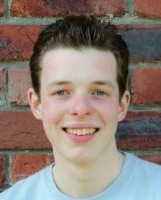
\includegraphics[height=3cm, width=10cm, keepaspectratio]{mitch}\\
Thiyanga Talagala & Pablo Montero-Manso\hspace*{-1cm} & Mitchell O'Hara-Wild
\end{tabular}

\end{block}

\end{frame}




\end{document}
